
\usetikzlibrary{arrows, positioning}
\subsubsection{Structure}
An Overview of the Hash Table.
Hash Functions.
Collisions Handling.
\begin{itemize}
    \item Direct Chaining (Sticking out)
    \item Linear Probing (Tucked in)
    \item Double Hashing (Tucked in)
\end{itemize}

\subsubsection{Overview}
Hash Table is an abstract data type that can map Keys to Values (key-value pairs).
Hash Table uses a hash function to calculate the index of a specific Key, and use this index (also called hash code) to locate the associated Value in an array of buckets or slots.
Hash Table must support three operations:
\begin{itemize}
    \item Insert
    \item Delete
    \item Lookup
\end{itemize}
Ideally the time complexity for these operations should be *amortized* $O(1)$.

\subsection*{Overview – Problems of Direct Address Table}
Assuming that a company has 4 employees, and their staff IDs contain 8 digitals.
E.g. 12345678.
In this case, the size of $U$ is $10^8 = 100,000,000$ and $K$ is 4!
Problems of Direct Address Table:
\begin{itemize}
    \item When $U$ is big, it consumes a lot of memories.
    \item When $U$ is big and $K$ is small, most of the slots will be Nil.
    \item So a large amount of space will be wasted.
    \item Cannot process Key-Value pairs where Keys are not digitals (e.g. ABCDEFGH, BCDEFGHI).
\end{itemize}

\textbf{Hash Table = DAT + Hashing + Collisions Handling} \\
\begin{tabular}{|l|l|}
\hline
Keys & Values \\
\hline
12343211 & Uday \\
12345678 & Niloofer \\
24283256 & Mirco \\
87654321 & Jizheng \\
\hline
\end{tabular}
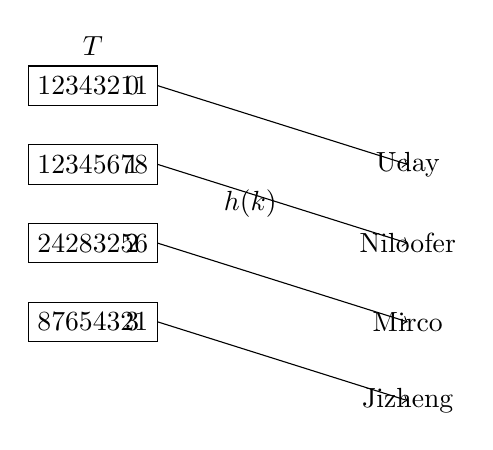
\begin{tikzpicture}
    \node at (0, 3) {$T$};
    \node[draw, minimum width=0.5cm, minimum height=0.5cm] (T0) at (0, 2.5) {12343211};
    \node[draw, minimum width=0.5cm, minimum height=0.5cm] (T1) at (0, 1.5) {12345678};
    \node[draw, minimum width=0.5cm, minimum height=0.5cm] (T2) at (0, 0.5) {24283256};
    \node[draw, minimum width=0.5cm, minimum height=0.5cm] (T3) at (0, -0.5) {87654321};
    \node at (0.5, 2.5) {0};
    \node at (0.5, 1.5) {1};
    \node at (0.5, 0.5) {2};
    \node at (0.5, -0.5) {3};
    \node at (2, 1) {$h(k)$};
    \node at (4, 1.5) {Uday};
    \node at (4, 0.5) {Niloofer};
    \node at (4, -0.5) {Mirco};
    \node at (4, -1.5) {Jizheng};

    \draw[->] (T0.east) -- (4, 1.5);
    \draw[->] (T1.east) -- (4, 0.5);
    \draw[->] (T2.east) -- (4, -0.5);
    \draw[->] (T3.east) -- (4, -1.5);
\end{tikzpicture}
$h(k)$ is a function that takes an input from $K$ and the output will be one of the indexes of $T$.

\subsubsection{Hash Function}
A hash function is any function that can be used to map data of arbitrary size to fixed-size values.
The values returned by a hash function are called Hash Codes.
Consider this as an Object that contains two fields “Key” and “Value”

\textbf{Hash Table = DAT + Hashing + Collisions Handling} \\
\begin{tabular}{|l|l|l|l|}
\hline
12343211 & 12345678 & 24283256 & 87654321 \\
\hline
\end{tabular}
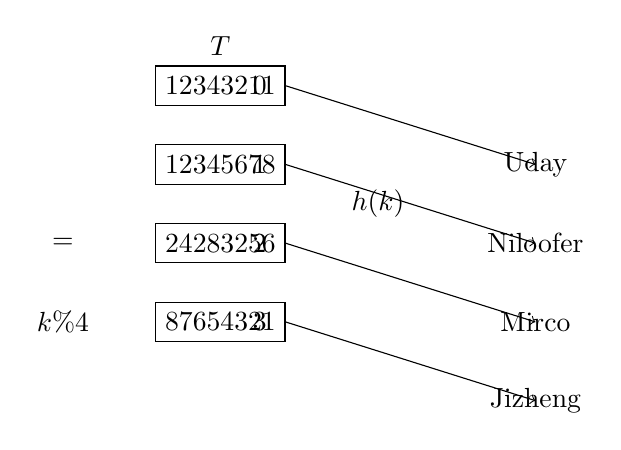
\begin{tikzpicture}
    \node at (0, 3) {$T$};
    \node[draw, minimum width=0.5cm, minimum height=0.5cm] (T0) at (0, 2.5) {12343211};
    \node[draw, minimum width=0.5cm, minimum height=0.5cm] (T1) at (0, 1.5) {12345678};
    \node[draw, minimum width=0.5cm, minimum height=0.5cm] (T2) at (0, 0.5) {24283256};
    \node[draw, minimum width=0.5cm, minimum height=0.5cm] (T3) at (0, -0.5) {87654321};
    \node at (0.5, 2.5) {0};
    \node at (0.5, 1.5) {1};
    \node at (0.5, 0.5) {2};
    \node at (0.5, -0.5) {3};
    \node at (2, 1) {$h(k)$};
    \node at (4, 1.5) {Uday};
    \node at (4, 0.5) {Niloofer};
    \node at (4, -0.5) {Mirco};
    \node at (4, -1.5) {Jizheng};

    \draw[->] (T0.east) -- (4, 1.5);
    \draw[->] (T1.east) -- (4, 0.5);
    \draw[->] (T2.east) -- (4, -0.5);
    \draw[->] (T3.east) -- (4, -1.5);

    \node at (-2, 0.5) {$=$};
    \node at (-2, -0.5) {$k\%4$};
\end{tikzpicture}
Modulus operator (\%): return the remainder or signed remainder of a division after one number is divided by another.
E.g:
$3\%4 = 3$
$4\%4 = 0$
$5\%4 = 1$
This is the most commonly used method for hashing Positive Integers, and is called modular hashing:
$h_k=k\%m$
where $m$ is the size of the array (or a prime which will be discussed later).
Discussion: Is it possible to handle negative integers with modular hashing?

Now Martin is coming….
\begin{tabular}{|l|l|}
\hline
Keys & Values \\
\hline
12343211 & Uday \\
12345678 & Niloofer \\
24283256 & Mirco \\
87654321 & Jizheng \\
12332121 & Martin \\
\hline
\end{tabular}
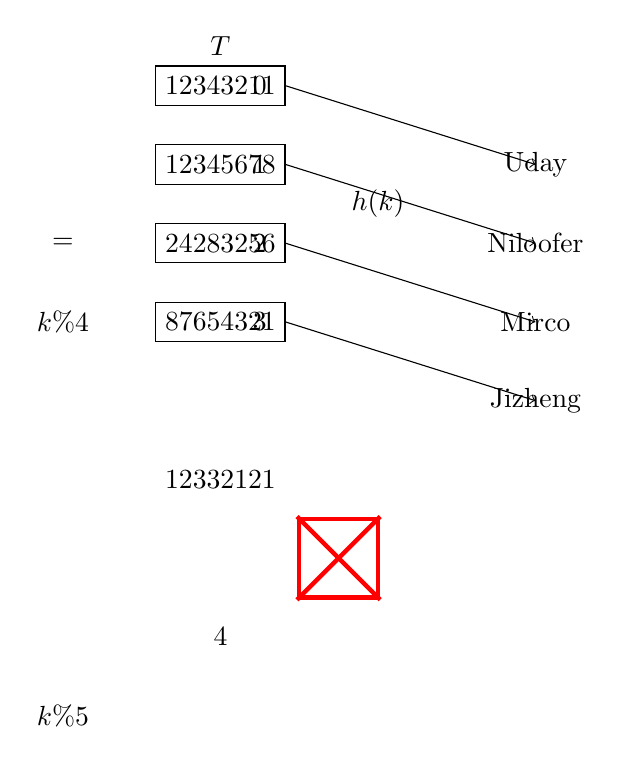
\begin{tikzpicture}
    \node at (0, 3) {$T$};
    \node[draw, minimum width=0.5cm, minimum height=0.5cm] (T0) at (0, 2.5) {12343211};
    \node[draw, minimum width=0.5cm, minimum height=0.5cm] (T1) at (0, 1.5) {12345678};
    \node[draw, minimum width=0.5cm, minimum height=0.5cm] (T2) at (0, 0.5) {24283256};
    \node[draw, minimum width=0.5cm, minimum height=0.5cm] (T3) at (0, -0.5) {87654321};
    \node at (0.5, 2.5) {0};
    \node at (0.5, 1.5) {1};
    \node at (0.5, 0.5) {2};
    \node at (0.5, -0.5) {3};
    \node at (2, 1) {$h(k)$};
    \node at (4, 1.5) {Uday};
    \node at (4, 0.5) {Niloofer};
    \node at (4, -0.5) {Mirco};
    \node at (4, -1.5) {Jizheng};

    \draw[->] (T0.east) -- (4, 1.5);
    \draw[->] (T1.east) -- (4, 0.5);
    \draw[->] (T2.east) -- (4, -0.5);
    \draw[->] (T3.east) -- (4, -1.5);

    \node at (-2, 0.5) {$=$};
    \node at (-2, -0.5) {$k\%4$};

    \node at (0, -2.5) {12332121};
    \node at (0, -3.5) {};
    \node at (0, -4.5) {4};
    \node at (-2, -5.5) {$k\%5$};
    \node[draw, red, ultra thick, minimum width=1cm, minimum height=1cm] (cross) at (1.5, -3.5) {};
    \draw[red, ultra thick] (cross.south west) -- (cross.north east);
    \draw[red, ultra thick] (cross.north west) -- (cross.south east);
\end{tikzpicture}

\begin{tabular}{|l|l|}
\hline
Keys & Values \\
\hline
12343211 & Uday \\
12345678 & Niloofer \\
24283256 & Mirco \\
87654321 & Jizheng \\
12332121 & Martin \\
\hline
\end{tabular}
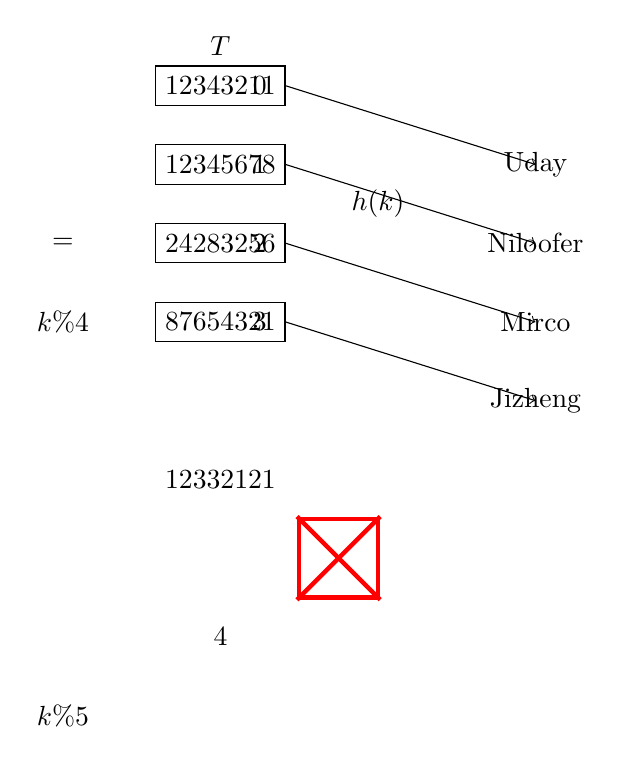
\begin{tikzpicture}
    \node at (0, 3) {$T$};
    \node[draw, minimum width=0.5cm, minimum height=0.5cm] (T0) at (0, 2.5) {12343211};
    \node[draw, minimum width=0.5cm, minimum height=0.5cm] (T1) at (0, 1.5) {12345678};
    \node[draw, minimum width=0.5cm, minimum height=0.5cm] (T2) at (0, 0.5) {24283256};
    \node[draw, minimum width=0.5cm, minimum height=0.5cm] (T3) at (0, -0.5) {87654321};
    \node at (0.5, 2.5) {0};
    \node at (0.5, 1.5) {1};
    \node at (0.5, 0.5) {2};
    \node at (0.5, -0.5) {3};
    \node at (2, 1) {$h(k)$};
    \node at (4, 1.5) {Uday};
    \node at (4, 0.5) {Niloofer};
    \node at (4, -0.5) {Mirco};
    \node at (4, -1.5) {Jizheng};

    \draw[->] (T0.east) -- (4, 1.5);
    \draw[->] (T1.east) -- (4, 0.5);
    \draw[->] (T2.east) -- (4, -0.5);
    \draw[->] (T3.east) -- (4, -1.5);

    \node at (-2, 0.5) {$=$};
    \node at (-2, -0.5) {$k\%4$};

    \node at (0, -2.5) {12332121};
    \node at (0, -3.5) {};
    \node at (0, -4.5) {4};
    \node at (-2, -5.5) {$k\%5$};
    \node[draw, red, ultra thick, minimum width=1cm, minimum height=1cm] (cross) at (1.5, -3.5) {};
    \draw[red, ultra thick] (cross.south west) -- (cross.north east);
    \draw[red, ultra thick] (cross.north west) -- (cross.south east);
\end{tikzpicture}

\subsection*{Hash Collisions}
Collisions are inevitable in Hash Table, so we need a mechanism to deal with hash collisions.
Hash Table = DAT + Hashing + Collisions Handling
\subsection*{Hash Functions}
The main purpose of the Hash Function is to produce Hash Codes based on the Keys.
Then use Hash Codes to index a Hash Table.

So what is a good Hash Function?
\begin{itemize}
    \item Deterministic – Equal keys must produce the same hash value.
    \item Efficient to compute.
    \item Uniformly distribute the key.
\end{itemize}
In other words, given a random Key, it ought to have the same probability of being stored on every position.

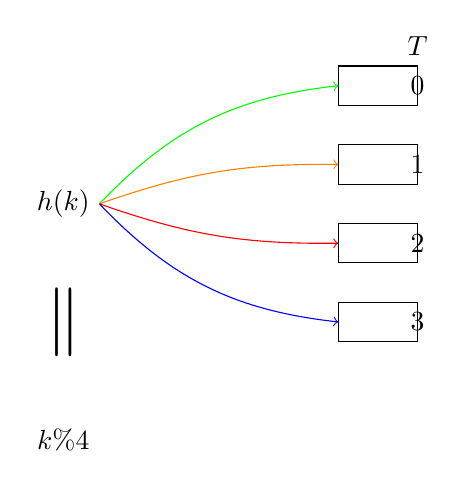
\begin{tikzpicture}
    \node at (-2, 0) (hk) {$h(k)$};
    \node at (-2, -1.5) (eq) {\Huge $\|$};
    \node at (-2, -3) (kmod4) {$k\%4$};
    \node[draw, minimum width=1cm, minimum height=0.5cm] (T0) at (2, 1.5) {};
    \node[draw, minimum width=1cm, minimum height=0.5cm] (T1) at (2, 0.5) {};
    \node[draw, minimum width=1cm, minimum height=0.5cm] (T2) at (2, -0.5) {};
    \node[draw, minimum width=1cm, minimum height=0.5cm] (T3) at (2, -1.5) {};

    \node at (2.5, 1.5) {0};
    \node at (2.5, 0.5) {1};
    \node at (2.5, -0.5) {2};
    \node at (2.5, -1.5) {3};
    \node at (2.5, 2) {$T$};

    \draw[->, green] (hk.east) to[bend left=20] (T0.west);
    \draw[->, orange] (hk.east) to[bend left=10] (T1.west);
    \draw[->, red] (hk.east) to[bend right=10] (T2.west);
    \draw[->, blue] (hk.east) to[bend right=20] (T3.west);
\end{tikzpicture}

Bad
Good
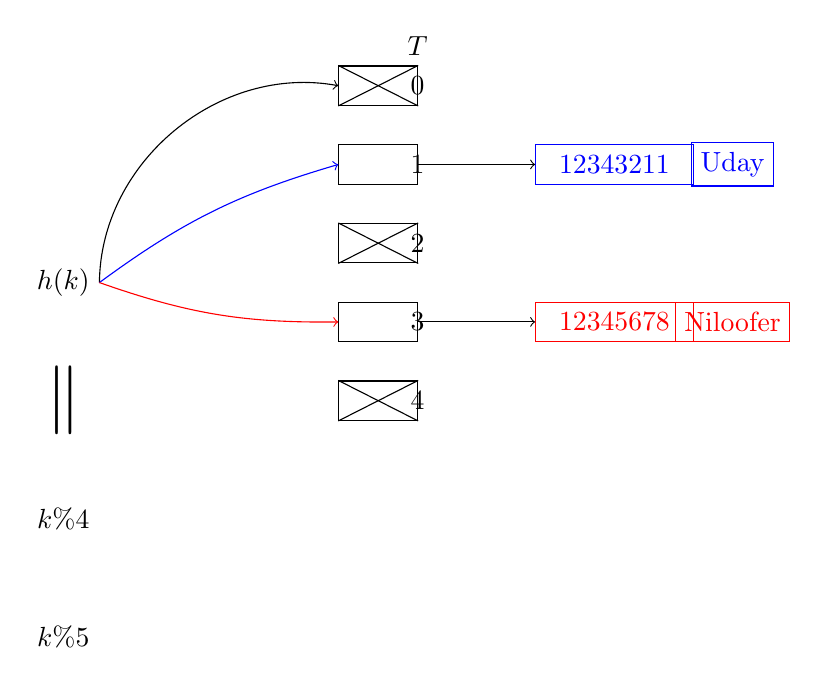
\begin{tikzpicture}
    \node at (-2, 0) (hk) {$h(k)$};
    \node at (-2, -1.5) (eq) {\Huge $\|$};
    \node at (-2, -3) (kmod4) {$k\%4$};
    \node at (-2, -4.5) (kmod5) {$k\%5$};

    \node[draw, minimum width=1cm, minimum height=0.5cm] (T0) at (2, 2.5) {};
    \node[draw, minimum width=1cm, minimum height=0.5cm] (T1) at (2, 1.5) {};
    \node[draw, minimum width=1cm, minimum height=0.5cm] (T2) at (2, 0.5) {};
    \node[draw, minimum width=1cm, minimum height=0.5cm] (T3) at (2, -0.5) {};
    \node[draw, minimum width=1cm, minimum height=0.5cm] (T4) at (2, -1.5) {};

    \node at (2.5, 2.5) {0};
    \node at (2.5, 1.5) {1};
    \node at (2.5, 0.5) {2};
    \node at (2.5, -0.5) {3};
    \node at (2.5, -1.5) {4};
    \node at (2.5, 3) {$T$};

    \draw (T0.south west) -- (T0.north east);
    \draw (T0.north west) -- (T0.south east);
    \draw (T2.south west) -- (T2.north east);
    \draw (T2.north west) -- (T2.south east);
    \draw (T4.south west) -- (T4.north east);
    \draw (T4.north west) -- (T4.south east);

    \draw[->] (hk.east) to[bend left=50] (T0.west);
    \draw[->, blue] (hk.east) to[bend left=10] (T1.west);
    \draw[->, red] (hk.east) to[bend right=10] (T3.west);

    \node[draw, blue, minimum width=2cm, minimum height=0.5cm] (val1) at (5, 1.5) {12343211};
    \node[draw, blue, minimum width=1cm, minimum height=0.5cm] (name1) at (6.5, 1.5) {Uday};
    \draw[->] (T1.east) -- (val1.west);

    \node[draw, red, minimum width=2cm, minimum height=0.5cm] (val2) at (5, -0.5) {12345678};
    \node[draw, red, minimum width=1cm, minimum height=0.5cm] (name2) at (6.5, -0.5) {Niloofer};
    \draw[->] (T3.east) -- (val2.west);
\end{tikzpicture}

\subsection*{Hash Functions – Positive Integers \& Floating-point Numbers}
Positive Integers (e.g. 1, 2, 3) – Modular Hashing
$h_k=k\%m$, where $m$ is the size of the array.
Good practice: choose a prime table size.
Floating-point Numbers (e.g. 0.1, 0.2, 0.3)
In Java, it uses IEEE 754 floating-point standard to represent floating-point numbers.
Modular Hashing on the binary representation of the floating-point numbers.
 
Quick Discussion:
What if m has some common factors with k?
(e.g. both m and k are always even numbers)

\subsubsection{Hash Functions - Strings}
Strings
Characters can be represented by ASC II codes*.
E.g. \\
Jay => [74, 97, 121] \\
Uday => [85, 100, 97, 121] \\
Then we can use the following formular to calculate the hash code: \\
\[
h=A^{n-1} \times s_0 + A^{n-2} \times s_1 + \dots + A^0 \times s[n-1]
\]
where $s[i]$ is the i-th ASC II code (decimal) in the string, $n$ is the length of the string and $A$ is a number.
For example: Let $A=2$, then:
$h_{Jay}=2^2 \times 74 + 2 \times 97 + 121 = 611$ \\
$h_{Uday}=2^3 \times 85 + 2^2 \times 100 + 2 \times 97 + 121 = 1395$ \\
 
ASCII, stands for American Standard Code for Information Interchange.
It's a 7-bit character code where every single bit represents a unique character \\
\begin{tabular}{|l|l|l|}
\hline
Decimal & Binary & Symbol \\
\hline
65 & 01000001 & A \\
66 & 01000010 & B \\
\ldots & \ldots & \ldots \\
90 & 01011010 & Z \\
\ldots & \ldots & \ldots \\
97 & 01100001 & a \\
\ldots & \ldots & \ldots \\
122 & 01111010 & z \\
\hline
\end{tabular}

Ideally, an odd prime number that is not too big or too small. \\
(so, 2 is, in fact, a bad choice!) \\
Too small => $A^{n-1}$ is going to be small when the string is short. \\
Hence, intuitively, the distribution will be squeezed into a relatively “small” range.
Too large => Integer overflow! \\
In Java, the max integer value (32-bits) is $2^{31}-1$. \\
 
How it has been done in Java?
\begin{lstlisting}
public static int hashCode(byte[] value) { 
    int h = 0;
    for (byte v : value) { 
        h = 31 * h + (v \& 0xff);
    }
    return h;
}
\end{lstlisting}

$h=31^{n-1} \times s_0 + 31^{n-2} \times s_1 + \dots + 31^0 \times s[n-1]$ \\
$h_{Jay}=31^2 \times 74 + 31 \times 97 + 121=74242$ \\
$h_{Jay}=((31 \times 0 + 74 )\times 31 + 97 )\times 31 + 121=74242$ \\

\subsection*{Shift Operator/Bit Shift}
Inside a computer, data has been stored in binary format.
\begin{tabular}{|l|l|l|}
\hline
0 & 00000000 & \\
1 & 00000001 & \\
2 & 00000010 & \\
8 & 00001000 & \\
4 & 00000100 & \\
\hline
\end{tabular}
Bitwise Left Shift Operator (\texttt{<<}) moves the binary numbers to the left and use 0 to fill the empty space.
Bitwise Right Shift Operator (\texttt{>>}) moves the binary numbers to the right and use 0 to fill the empty space.
$1 \ll 1 =$
$8 \gg 1 =$
In fact, $i \times 2 = i \ll 1$ and $i \div 2 = i \gg 1$, and use shift operator is much faster than the $\times$ and $\div$ operations.
\begin{tabular}{|l|l|}
\hline
0 & 00000010 \\
0 & 00000100 \\
\hline
\end{tabular}

\subsection{Collisions Handling}
Hash Collisions means the hash function generates the same index for more than one key.
Two types of strategies:
\begin{itemize}
    \item Sticking out (Chaining).
    \item Tucked in (Open Addressing).
\end{itemize}

\begin{tikzpicture}
    % Sticking out
    \node at (-3, 3) {$T$};
    \node[draw, minimum width=0.5cm, minimum height=0.5cm] (Tso0) at (-3, 2.5) {};
    \node[draw, minimum width=0.5cm, minimum height=0.5cm] (Tso1) at (-3, 1.5) {};
    \node[draw, minimum width=0.5cm, minimum height=0.5cm] (Tso2) at (-3, 0.5) {};
    \node[draw, minimum width=0.5cm, minimum height=0.5cm] (Tso3) at (-3, -0.5) {};
    \node[draw, minimum width=0.5cm, minimum height=0.5cm] (Tso4) at (-3, -1.5) {};
    \node[draw, minimum width=0.5cm, minimum height=0.5cm] (Tso5) at (-3, -2.5) {};
    \node[draw, minimum width=0.5cm, minimum height=0.5cm] (Tso6) at (-3, -3.5) {};
    \node[draw, minimum width=0.5cm, minimum height=0.5cm] (Tso7) at (-3, -4.5) {};
    \node at (-2.5, 2.5) {0};
    \node at (-2.5, 1.5) {1};
    \node at (-2.5, 0.5) {2};
    \node at (-2.5, -0.5) {3};
    \node at (-2.5, -1.5) {4};
    \node at (-2.5, -2.5) {5};
    \node at (-2.5, -3.5) {6};
    \node at (-2.5, -4.5) {7};

    \node at (-3, -6) {Sticking out};

    % Tucked in
    \node at (3, 3) {$T$};
    \node[draw, minimum width=0.5cm, minimum height=0.5cm] (Tti0) at (3, 2.5) {};
    \node[draw, minimum width=0.5cm, minimum height=0.5cm] (Tti1) at (3, 1.5) {};
    \node[draw, minimum width=0.5cm, minimum height=0.5cm] (Tti2) at (3, 0.5) {};
    \node[draw, minimum width=0.5cm, minimum height=0.5cm] (Tti3) at (3, -0.5) {};
    \node[draw, minimum width=0.5cm, minimum height=0.5cm] (Tti4) at (3, -1.5) {};
    \node[draw, minimum width=0.5cm, minimum height=0.5cm] (Tti5) at (3, -2.5) {};
    \node[draw, minimum width=0.5cm, minimum height=0.5cm] (Tti6) at (3, -3.5) {};
    \node[draw, minimum width=0.5cm, minimum height=0.5cm] (Tti7) at (3, -4.5) {};
    \node at (3.5, 2.5) {0};
    \node at (3.5, 1.5) {1};
    \node at (3.5, 0.5) {2};
    \node at (3.5, -0.5) {3};
    \node at (3.5, -1.5) {4};
    \node at (3.5, -2.5) {5};
    \node at (3.5, -3.5) {6};
    \node at (3.5, -4.5) {7};

    \node at (3, -6) {Tucked in};

    \node at (0, -7.5) {$k\%8$};

    % Values for Tucked In
    \node[right of=Tti1, node distance=1.5cm] (v9) {9};
    \node[right of=Tti4, node distance=1.5cm] (v12) {12};
    \node[right of=Tti5, node distance=1.5cm] (v28) {28};
    \node[right of=Tti6, node distance=1.5cm] (v14) {14};
    \node[right of=Tti7, node distance=1.5cm] (v30) {30};
    \node[right of=Tti0, node distance=1.5cm] (v25) {25};
\end{tikzpicture}

\subsubsection{Sticking out – Linked Lists}
Linked List is a sequence of nodes.
Each node contains two fields:
\begin{itemize}
    \item Data
    \item A link to the next node.
\end{itemize}

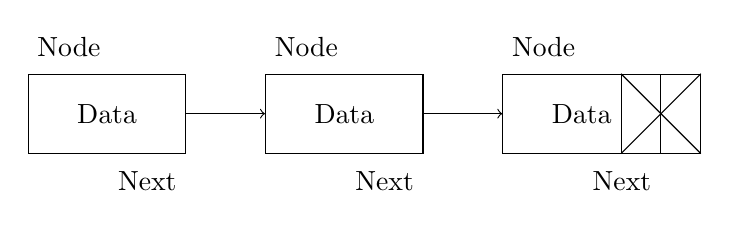
\begin{tikzpicture}
    \tikzstyle{nodebox}=[draw, minimum width=2cm, minimum height=1cm, rectangle]
    \tikzstyle{nullbox}=[draw, minimum width=1cm, minimum height=1cm, rectangle]

    \node[nodebox] (node1) {Data};
    \node[nodebox, right=of node1] (node2) {Data};
    \node[nodebox, right=of node2] (node3) {Data};

    \node[above=0.1cm of node1.north west, anchor=south west] {Node};
    \node[above=0.1cm of node2.north west, anchor=south west] {Node};
    \node[above=0.1cm of node3.north west, anchor=south west] {Node};

    \node[below=0.1cm of node1.south east, anchor=north east] {Next};
    \node[below=0.1cm of node2.south east, anchor=north east] {Next};
    \node[below=0.1cm of node3.south east, anchor=north east] {Next};

    \draw[->] (node1.east) -- (node2.west);
    \draw[->] (node2.east) -- (node3.west);

    \node[nullbox] (null) at (node3.east) {};
    \draw (null.south west) -- (null.north east);
    \draw (null.north west) -- (null.south east);
\end{tikzpicture}

\textbf{Sticking out – Linked Lists} \\
Different types of linked list:
\begin{itemize}
    \item Single linked list: Item navigation is forward only.
    \item Double linked list: Items can be navigated forward and backward.
    \item Circular linked list: The next link in the last node will point to the first node.
\end{itemize}

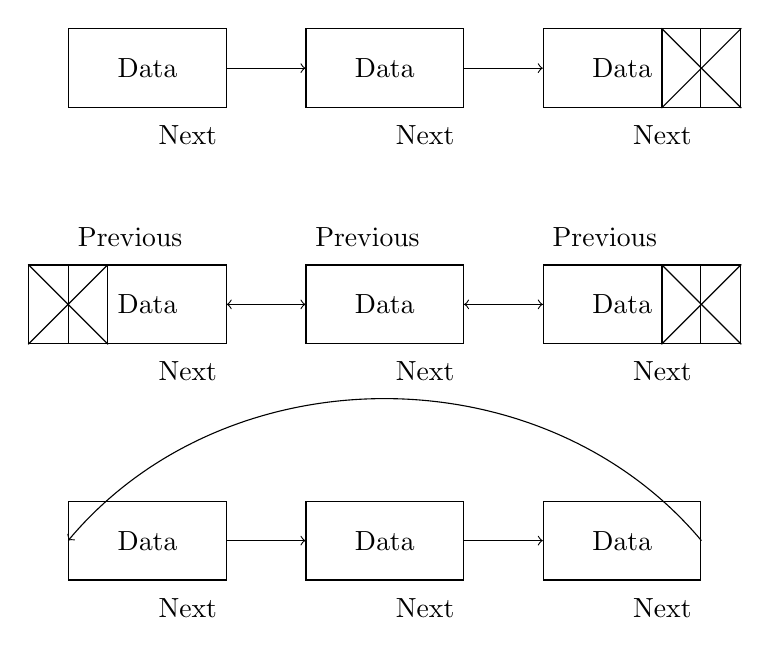
\begin{tikzpicture}
    \tikzstyle{nodebox}=[draw, minimum width=2cm, minimum height=1cm, rectangle]
    \tikzstyle{nullbox}=[draw, minimum width=1cm, minimum height=1cm, rectangle]

    % Single Linked List
    \node[nodebox] (s_node1) at (0, 0) {Data};
    \node[nodebox, right=of s_node1] (s_node2) {Data};
    \node[nodebox, right=of s_node2] (s_node3) {Data};

    \node[below=0.1cm of s_node1.south east, anchor=north east] {Next};
    \node[below=0.1cm of s_node2.south east, anchor=north east] {Next};
    \node[below=0.1cm of s_node3.south east, anchor=north east] {Next};

    \draw[->] (s_node1.east) -- (s_node2.west);
    \draw[->] (s_node2.east) -- (s_node3.west);

    \node[nullbox] (s_null) at (s_node3.east) {};
    \draw (s_null.south west) -- (s_null.north east);
    \draw (s_null.north west) -- (s_null.south east);

    % Double Linked List
    \node[nodebox] (d_node1) at (0, -3) {Data};
    \node[nodebox, right=of d_node1] (d_node2) {Data};
    \node[nodebox, right=of d_node2] (d_node3) {Data};

    \node[below=0.1cm of d_node1.south east, anchor=north east] {Next};
    \node[above=0.1cm of d_node1.north west, anchor=south west] {Previous};
    \node[below=0.1cm of d_node2.south east, anchor=north east] {Next};
    \node[above=0.1cm of d_node2.north west, anchor=south west] {Previous};
    \node[below=0.1cm of d_node3.south east, anchor=north east] {Next};
    \node[above=0.1cm of d_node3.north west, anchor=south west] {Previous};

    \draw[->] (d_node1.east) -- (d_node2.west);
    \draw[->] (d_node2.east) -- (d_node3.west);
    \draw[->] (d_node2.west) -- (d_node1.east);
    \draw[->] (d_node3.west) -- (d_node2.east);

    \node[nullbox] (d_null1) at (d_node1.west) {};
    \draw (d_null1.south west) -- (d_null1.north east);
    \draw (d_null1.north west) -- (d_null1.south east);
    \node[nullbox] (d_null2) at (d_node3.east) {};
    \draw (d_null2.south west) -- (d_null2.north east);
    \draw (d_null2.north west) -- (d_null2.south east);

    % Circular Linked List
    \node[nodebox] (c_node1) at (0, -6) {Data};
    \node[nodebox, right=of c_node1] (c_node2) {Data};
    \node[nodebox, right=of c_node2] (c_node3) {Data};

    \node[below=0.1cm of c_node1.south east, anchor=north east] {Next};
    \node[below=0.1cm of c_node2.south east, anchor=north east] {Next};
    \node[below=0.1cm of c_node3.south east, anchor=north east] {Next};

    \draw[->] (c_node1.east) -- (c_node2.west);
    \draw[->] (c_node2.east) -- (c_node3.west);
    \draw[->] (c_node3.east) to[bend right=50] (c_node1.west);
\end{tikzpicture}

\subsubsection{Sticking out – Linked Lists}
Basic Operations (single linked list):
\begin{itemize}
    \item Insertion: $O(1)$ or $O(n)$
    \item Deletion: $O(1)$ or $O(n)$
    \item Search: $O(n)$
\end{itemize}

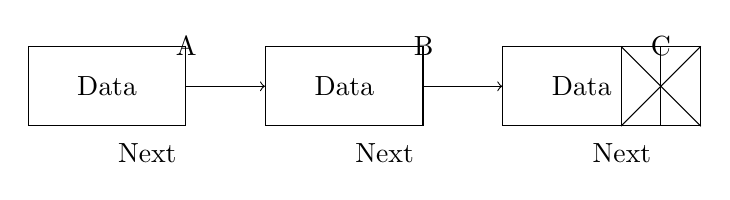
\begin{tikzpicture}
    \tikzstyle{nodebox}=[draw, minimum width=2cm, minimum height=1cm, rectangle]
    \tikzstyle{nullbox}=[draw, minimum width=1cm, minimum height=1cm, rectangle]

    \node[nodebox] (nodeA) at (0, 0) {Data};
    \node[nodebox, right=of nodeA] (nodeB) {Data};
    \node[nodebox, right=of nodeB] (nodeC) {Data};

    \node[below=0.1cm of nodeA.south east, anchor=north east] {Next};
    \node[below=0.1cm of nodeB.south east, anchor=north east] {Next};
    \node[below=0.1cm of nodeC.south east, anchor=north east] {Next};

    \node at (nodeA.north east) {A};
    \node at (nodeB.north east) {B};
    \node at (nodeC.north east) {C};

    \draw[->] (nodeA.east) -- (nodeB.west);
    \draw[->] (nodeB.east) -- (nodeC.west);

    \node[nullbox] (null) at (nodeC.east) {};
    \draw (null.south west) -- (null.north east);
    \draw (null.north west) -- (null.south east);
\end{tikzpicture}
Insertion
Time Complexity:
\begin{itemize}
    \item Insert after the current node or at the beginning of the list: $O(1)$
    \item Anywhere else: $O(n)$
\end{itemize}
 

\subsubsection{Sticking out – Linked Lists}
Basic Operations (single linked list):
\begin{itemize}
    \item Insertion: $O(1)$ or $O(n)$
    \item Deletion: $O(1)$ or $O(n)$
    \item Search: $O(n)$
\end{itemize}
 
Deletion
Time Complexity:
\begin{itemize}
    \item Delete after the current node or at the beginning of the list: $O(1)$
    \item Anywhere else: $O(n)$
\end{itemize}
 
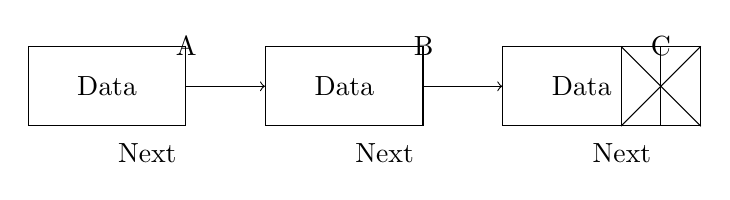
\begin{tikzpicture}
    \tikzstyle{nodebox}=[draw, minimum width=2cm, minimum height=1cm, rectangle]
    \tikzstyle{nullbox}=[draw, minimum width=1cm, minimum height=1cm, rectangle]

    \node[nodebox] (nodeA) at (0, 0) {Data};
    \node[nodebox, right=of nodeA] (nodeB) {Data};
    \node[nodebox, right=of nodeB] (nodeC) {Data};

    \node[below=0.1cm of nodeA.south east, anchor=north east] {Next};
    \node[below=0.1cm of nodeB.south east, anchor=north east] {Next};
    \node[below=0.1cm of nodeC.south east, anchor=north east] {Next};

    \node at (nodeA.north east) {A};
    \node at (nodeB.north east) {B};
    \node at (nodeC.north east) {C};

    \draw[->] (nodeA.east) -- (nodeB.west);
    \draw[->] (nodeB.east) -- (nodeC.west);

    \node[nullbox] (null) at (nodeC.east) {};
    \draw (null.south west) -- (null.north east);
    \draw (null.north west) -- (null.south east);
\end{tikzpicture}

\subsubsection{Sticking out – Direct Chaining}
\begin{tabular}{|l|l|l|l|l|l|l|l|}
\hline
Key & 8 & 11 & 13 & 15 & 20 & 25 & 30 \\
\hline
Value & Uday & Mian & Mirco & Jizheng & Martin & Mark & Peter \\
\hline
Hash Code & 1 & 4 & 6 & 1 & 6 & 4 & 2 \\
\hline
\end{tabular}
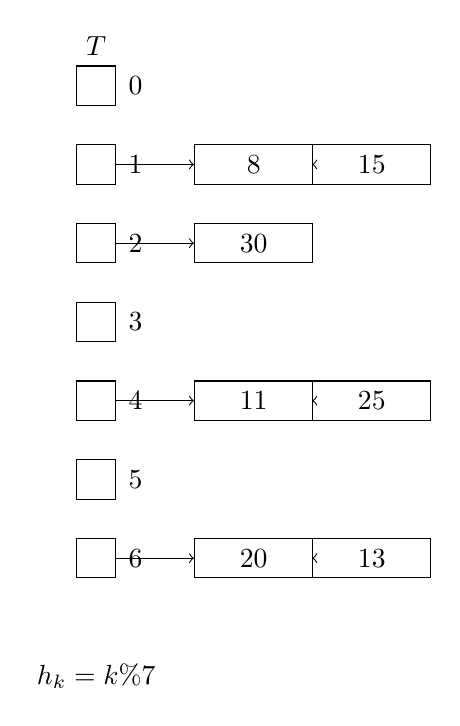
\begin{tikzpicture}
    \node at (0, 3) {$T$};
    \node[draw, minimum width=0.5cm, minimum height=0.5cm] (T0) at (0, 2.5) {};
    \node[draw, minimum width=0.5cm, minimum height=0.5cm] (T1) at (0, 1.5) {};
    \node[draw, minimum width=0.5cm, minimum height=0.5cm] (T2) at (0, 0.5) {};
    \node[draw, minimum width=0.5cm, minimum height=0.5cm] (T3) at (0, -0.5) {};
    \node[draw, minimum width=0.5cm, minimum height=0.5cm] (T4) at (0, -1.5) {};
    \node[draw, minimum width=0.5cm, minimum height=0.5cm] (T5) at (0, -2.5) {};
    \node[draw, minimum width=0.5cm, minimum height=0.5cm] (T6) at (0, -3.5) {};
    \node at (0.5, 2.5) {0};
    \node at (0.5, 1.5) {1};
    \node at (0.5, 0.5) {2};
    \node at (0.5, -0.5) {3};
    \node at (0.5, -1.5) {4};
    \node at (0.5, -2.5) {5};
    \node at (0.5, -3.5) {6};

    \node at (0, -5) {$h_k=k\%7$};

    \node[draw, minimum width=1.5cm, minimum height=0.5cm] (node8) at (2, 1.5) {8};
    \node[draw, minimum width=1.5cm, minimum height=0.5cm] (node15) at (3.5, 1.5) {15};
    \node[draw, minimum width=1.5cm, minimum height=0.5cm] (node11) at (2, -1.5) {11};
    \node[draw, minimum width=1.5cm, minimum height=0.5cm] (node25) at (3.5, -1.5) {25};
    \node[draw, minimum width=1.5cm, minimum height=0.5cm] (node20) at (2, -3.5) {20};
    \node[draw, minimum width=1.5cm, minimum height=0.5cm] (node13) at (3.5, -3.5) {13};
    \node[draw, minimum width=1.5cm, minimum height=0.5cm] (node30) at (2, 0.5) {30};

    \draw[->] (T1.east) -- (node8.west);
    \draw[->] (T4.east) -- (node11.west);
    \draw[->] (T6.east) -- (node20.west);
    \draw[->] (T2.east) -- (node30.west);

    \draw[->] (node8.east) -- (node15.west);
    \draw[->] (node11.east) -- (node25.west);
    \draw[->] (node20.east) -- (node13.west);
\end{tikzpicture}

\textbf{Load Factor (L)} \\
Let $n$ be the total number of stored entries;
$T$ be the size of the hash table, then: $L=\frac{n}{T}$
 
\textbf{Rehashing} \\
If the load factor (L) is bigger than a threshold ($\lambda$), then double the size of the hash table (T) , and hashing the table again.
Time complexity for rehashing is $O(N)$.
In Java, $\lambda = 0.75$.

\textbf{Sticking out – Direct Chaining} \\
Lookup Operation
Unsuccessful lookup
Key is not in the table.
On average, each chain contains $\frac{n}{T}$ Key-Value pairs.
We have to traverse $(\frac{n}{T})$.
Successful lookup
Key is in the table.
On average, each chain contains $\frac{n}{T}$ Key-Value pairs.
The expected position of Key in the chain is in the middle.
On average, need to traverse $\frac{1}{2}(1+\frac{n}{T})$ pairs.

Time Complexity (amortized)
Unsuccessful lookup:
$\frac{n}{T}=L \le \lambda \quad ===> \quad O(1)$
Successful lookup:
$\frac{1}{2}(1+L) \le \frac{1}{2}(1+\lambda) \quad ===> \quad O(1)$ \\

Insertion Time Complexity
Check if the Key is stored in the table, which is same as unsuccessful lookup: $\frac{n}{T}$.
If it is not, append the Key at the beginning of the associated link: 1.
In total: $\frac{n}{T}+1 \le \lambda+1 \quad ===> \quad O(1)$
Deletion Time Complexity
Same as successful lookup: $O(1)$
 
\textbf{Sticking out – Direct Chaining} \\
Advantage:
\begin{itemize}
    \item Easy to implement.
    \item Easy to understand – If a pair exist in the hash table, then it will only be found in the linked list.
\end{itemize}
Disadvantages:
\begin{itemize}
    \item Typically, there is a lot of hash collisions, therefore a lot of unused space.
    \item Linked lists require a lot of memory allocations, which is slow.
\end{itemize}

\textbf{Tucked in/Open Addressing - Linear probing} \\
\begin{tabular}{|l|l|l|l|l|l|l|l|}
\hline
Key & 8 & 11 & 13 & 15 & 20 & 25 & 30 \\
\hline
Value & Uday & Mian & Mirco & Jizheng & Martin & Mark & Peter \\
\hline
Hash Code & 1 & 4 & 6 & 1 & 6 & 4 & 2 \\
\hline
\end{tabular}
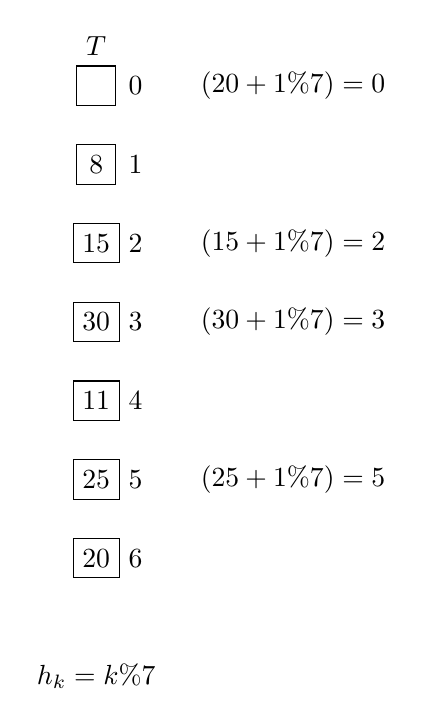
\begin{tikzpicture}
    \node at (0, 3) {$T$};
    \node[draw, minimum width=0.5cm, minimum height=0.5cm] (T0) at (0, 2.5) {};
    \node[draw, minimum width=0.5cm, minimum height=0.5cm] (T1) at (0, 1.5) {8};
    \node[draw, minimum width=0.5cm, minimum height=0.5cm] (T2) at (0, 0.5) {15};
    \node[draw, minimum width=0.5cm, minimum height=0.5cm] (T3) at (0, -0.5) {30};
    \node[draw, minimum width=0.5cm, minimum height=0.5cm] (T4) at (0, -1.5) {11};
    \node[draw, minimum width=0.5cm, minimum height=0.5cm] (T5) at (0, -2.5) {25};
    \node[draw, minimum width=0.5cm, minimum height=0.5cm] (T6) at (0, -3.5) {20};
    \node at (0.5, 2.5) {0};
    \node at (0.5, 1.5) {1};
    \node at (0.5, 0.5) {2};
    \node at (0.5, -0.5) {3};
    \node at (0.5, -1.5) {4};
    \node at (0.5, -2.5) {5};
    \node at (0.5, -3.5) {6};

    \node at (0, -5) {$h_k=k\%7$};

    \node at (2.5, 0.5) {$(15+1\%7)=2$};
    \node at (2.5, 2.5) {$(20+1\%7)=0$};
    \node at (2.5, -2.5) {$(25+1\%7)=5$};
    \node at (2.5, -0.5) {$(30+1\%7)=3$};
\end{tikzpicture} \\
\textbf{Insertion:} \\
If the primary position is occupied, search for the next available position by calculating $k+i\%T$, where $i=1,2,3\ldots$, $T$ is the hash table size.

\begin{tabular}{|l|l|l|l|l|l|l|l|}
\hline
Key & 8 & 11 & 13 & 15 & 20 & 25 & 30 \\
\hline
Value & Uday & Mian & Mirco & Jizheng & Martin & Mark & Peter \\
\hline
Hash Code & 1 & 4 & 6 & 1 & 6 & 4 & 2 \\
\hline
\end{tabular}
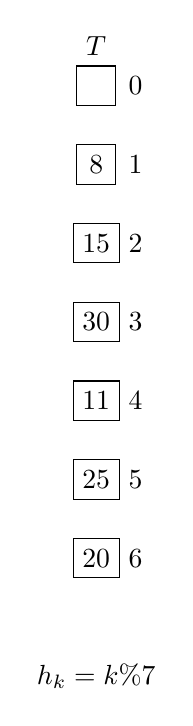
\begin{tikzpicture}
    \node at (0, 3) {$T$};
    \node[draw, minimum width=0.5cm, minimum height=0.5cm] (T0) at (0, 2.5) {};
    \node[draw, minimum width=0.5cm, minimum height=0.5cm] (T1) at (0, 1.5) {8};
    \node[draw, minimum width=0.5cm, minimum height=0.5cm] (T2) at (0, 0.5) {15};
    \node[draw, minimum width=0.5cm, minimum height=0.5cm] (T3) at (0, -0.5) {30};
    \node[draw, minimum width=0.5cm, minimum height=0.5cm] (T4) at (0, -1.5) {11};
    \node[draw, minimum width=0.5cm, minimum height=0.5cm] (T5) at (0, -2.5) {25};
    \node[draw, minimum width=0.5cm, minimum height=0.5cm] (T6) at (0, -3.5) {20};
    \node at (0.5, 2.5) {0};
    \node at (0.5, 1.5) {1};
    \node at (0.5, 0.5) {2};
    \node at (0.5, -0.5) {3};
    \node at (0.5, -1.5) {4};
    \node at (0.5, -2.5) {5};
    \node at (0.5, -3.5) {6};

    \node at (0, -5) {$h_k=k\%7$};
\end{tikzpicture} \\
\textbf{Deletion:} \\
Find whether the Key is stored in the table.
If it is, replace it with a tombstone (\#).
Search
Starting from the primary position, if it is the correct Key, stop.
Otherwise, keep moving to the next available position (skip over all tombstones).
If we reach an empty position, then the Key is not in the table, because every position is either empty, or it stores a tombstone, or a key.
Time Complexity: $O(1)$
 
\subsubsection{Tucked in/Open Addressing – Double hashing}
\begin{tabular}{|l|l|l|l|l|l|l|l|}
\hline
Key & 8 & 11 & 13 & 15 & 20 & 25 & 30 \\
\hline
Value & Uday & Mian & Mirco & Jizheng & Martin & Mark & Peter \\
\hline
Hash Code & 1 & 4 & 6 & 1 & 6 & 4 & 2 \\
\hline
\end{tabular} 

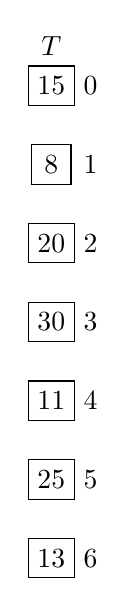
\begin{tikzpicture}
    \node at (0, 3) {$T$};
    \node[draw, minimum width=0.5cm, minimum height=0.5cm] (T0) at (0, 2.5) {15};
    \node[draw, minimum width=0.5cm, minimum height=0.5cm] (T1) at (0, 1.5) {8};
    \node[draw, minimum width=0.5cm, minimum height=0.5cm] (T2) at (0, 0.5) {20};
    \node[draw, minimum width=0.5cm, minimum height=0.5cm] (T3) at (0, -0.5) {30};
    \node[draw, minimum width=0.5cm, minimum height=0.5cm] (T4) at (0, -1.5) {11};
    \node[draw, minimum width=0.5cm, minimum height=0.5cm] (T5) at (0, -2.5) {25};
    \node[draw, minimum width=0.5cm, minimum height=0.5cm] (T6) at (0, -3.5) {13};
    \node at (0.5, 2.5) {0};
    \node at (0.5, 1.5) {1};
    \node at (0.5, 0.5) {2};
    \node at (0.5, -0.5) {3};
    \node at (0.5, -1.5) {4};
    \node at (0.5, -2.5) {5};
    \node at (0.5, -3.5) {6};
\end{tikzpicture}

\begin{math}
    h_1(k)=k\%7   \\
    h_2(k)=3-(k\%3) \\
    h_{(k,i)}=[h_1(k)+i \times h_2(k)]\%7 \\
    \\
    h(8,0) = [8\%7+0 \times (3-8\%3)]\%7 = 1\%7 = 1 \\
    h(11,0) = [11\%7+0 \times (3-11\%3)]\%7 = 4\%7 = 4 \\
    h(13,0) = [13\%7+0 \times (3-13\%3)]\%7 = 6\%7 = 6 \\
    h(15,0) = [15\%7+0 \times (3-15\%3)]\%7  = 1\%7 = 1 \\
    h(15,1) = [15\%7+1 \times (3-15\%3)]\%7 = (1+3)\%7 = 4 \\
    h(15,2) = [15\%7+2 \times (3-15\%3)]\%7 = (1+6)\%7 = 0 \\
    h(20,0) = [20\%7+0 \times (3-20\%3)]\%7 = 6\%7 = 6 \\
    h(20,1) = [20\%7+1 \times (3-20\%3)]\%7 = (6+1)\%7 = 0 \\
    h(20,2) = [20\%7+2 \times (3-20\%3)]\%7 = (6+2)\%7 = 1 \\
    h(20,3) = [20\%7+3 \times (3-20\%3)]\%7 = (6+3)\%7 = 2 \\
\end{math} 
\textbf{Short Cycle Solution} \\
$T$ is a prime number.
$T=2^k$ and $h_2$ is always an odd number.
 
Hash Table size $T$ and $h_2$ have to be coprime!

\subsubsection{Summary}
Hash tables consist of an array, a primary hash function $h_1$ (and secondary hash function $h_2$).
All operations are in $O(1)$ (amortized time) if:
\begin{itemize}
    \item $h_1$ (and $h_2$) computes indexes uniformly,
    \item Rehash whenever the table becomes full,
    \item ($T=2^k$ for some $k$, and $h_2$ gives odd numbers).
\end{itemize}

\subsection{Quicksort}

\textbf{Key steps:}
\begin{enumerate}
  \item Select an element from an array, called Pivot.
  \item Partition the array by moving all elements that are smaller than the Pivot to the left side of the Pivot, and all elements that are bigger than the Pivot to the right side of the Pivot.
  \item Apply Step 1 and 2 recursively until the whole array get sorted.
\end{enumerate}

\textbf{Detailed Steps} 
\begin{enumerate}[label=\arabic*:]
  \item Let the Pivot (P) be the last element of the array.
  \item 
  \begin{enumerate}[label*=\arabic*.]
    \item Let the Left Pointer (L) be the value of the first index of the array, and the Right Pointer (R) be the value of the last index of the array.
    \item Go through the array and move L (from left to right) to the first element in the array that is bigger than P (if L $\geq$ R, stop).
    \item Then move R (from right to left) to the first element that is smaller than P (if L $\geq$ R, stop).
    \item Swap the value of L and R.
    \item Repeat 2.2 to 2.4, until L $\geq$ R. Then swap L and P.
  \end{enumerate}
  \item Now the array has been split into two parts: Everything to the left of P is smaller than the value of P, while everything to the right of P is bigger than P. Repeat the same process on these two parts until the whole array get sorted.
\end{enumerate}


\textbf{Example:}

\begin{center}
Original Array: 20, 15, 10, 50, 16, 18
\end{center}

\begin{itemize}
  \item P = 18, L = 20, R = 18
  \item Start to move L. 20 > 18, stop L, and start to move R.
  \item 16 < 18, stop R. Swap L and R.
  \item Move L to the 15. 15 < 18, keep moving. 10 < 18, keep moving, 50 > 18, stop L and start to move R.
  \item Both L and R point to 50, swap 50 and 18.
  \item ...
  \item Final sorted: \{10, 15, 16, 18, 20, 50\}
\end{itemize}

\textbf{Remark:} Move R first if Pivot is the first element of the array.

\subsubsection{Time Complexity}
\begin{itemize}
  \item Partitioning/Splitting: $O(\log n)$ if pivot is in the middle.
  \item Swapping/Merging: $O(n)$
  \item \textbf{Overall:}
  \begin{itemize}
    \item On average: $O(n \log n)$
    \item Worst case: $O(n^2)$ e.g. nearly sorted array using first/last as pivot
  \end{itemize}
  \item Space Complexity: $O(\log n)$
\end{itemize}

\subsection{Heapsort}

\textbf{Priority Queue (PQ)}
\begin{itemize}
  \item PQ is an abstract data type, where each element has a “priority”.
  \item Priority is determined by the value (e.g. max or min).
  \item Supports operations:
  \begin{itemize}
    \item is\_empty
    \item insert
    \item pull
  \end{itemize}
\end{itemize}

\textbf{Complete Binary Tree} \\
A complete binary tree is a binary tree in which every level, except possibly the last, is completely filled, and all nodes are as far left as possible.
\begin{center}
    \begin{figure}[!htbp]
      \centering
      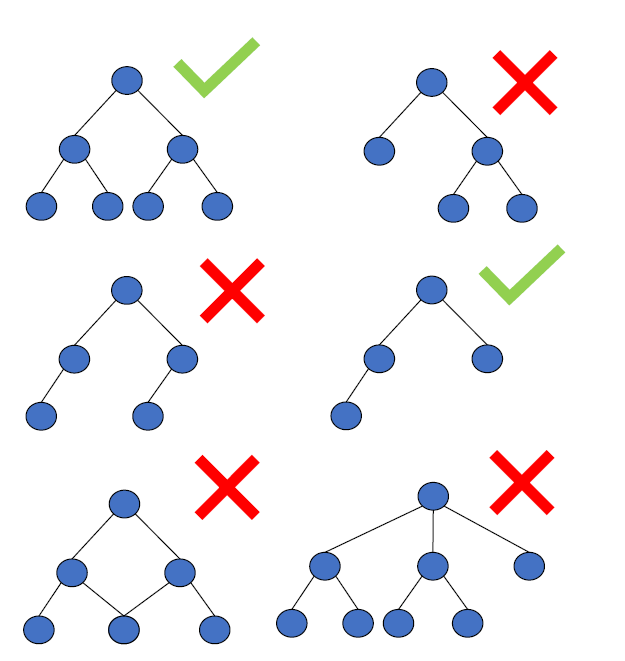
\includegraphics[width=8cm]{unit-5/figures/complete_binary_tree.png}
      \caption*{Complete Binary Tree}
    \end{figure}
\end{center}

\textbf{Binary Heap} \\
Binary Heap is a Complete Binary Tree which satisfies the heap property:

\begin{figure}[!htbp]
    \centering
    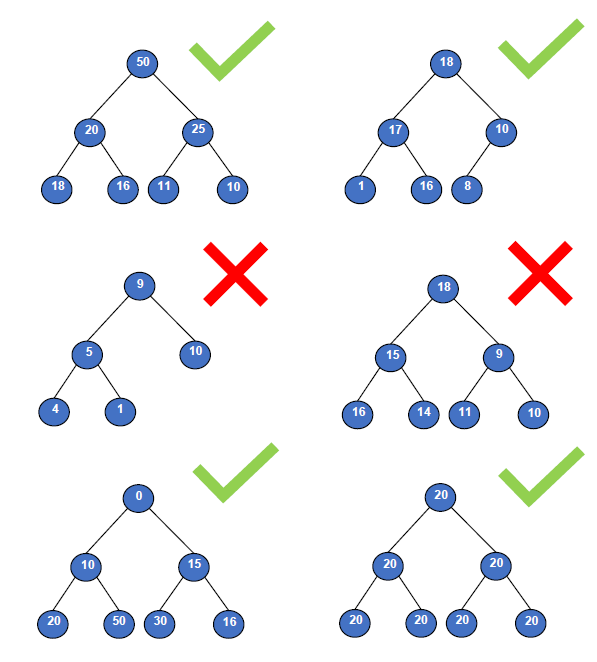
\includegraphics[width=10cm]{unit-5/figures/binary_heap.png}
    \caption*{Binary Heap}
\end{figure}

\begin{itemize}
  \item Max-Heap: parent $\geq$ children
  \item Min-Heap: parent $\leq$ children
\end{itemize}

\textbf{Heap and Array Mapping}

\begin{figure}[!htbp]
    \centering
    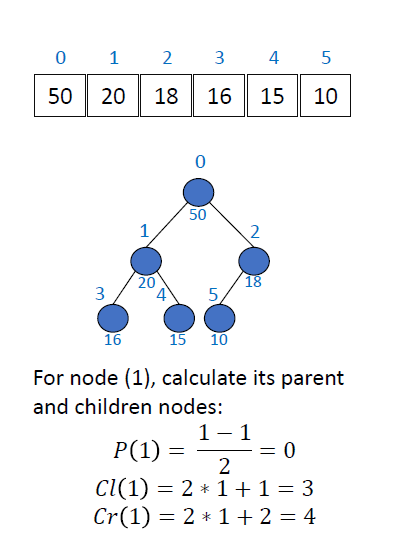
\includegraphics[width=10cm]{unit-5/figures/build_binary_heap.png}
    % \caption*{Binary Heap}
\end{figure}
\[
P(i) = \left\lfloor \frac{i - 1}{2} \right\rfloor, \quad C_l(i) = 2i + 1, \quad C_r(i) = 2i + 2
\]

\textbf{Build Max-Heap} \\

\begin{figure}[!htbp]
    \centering
    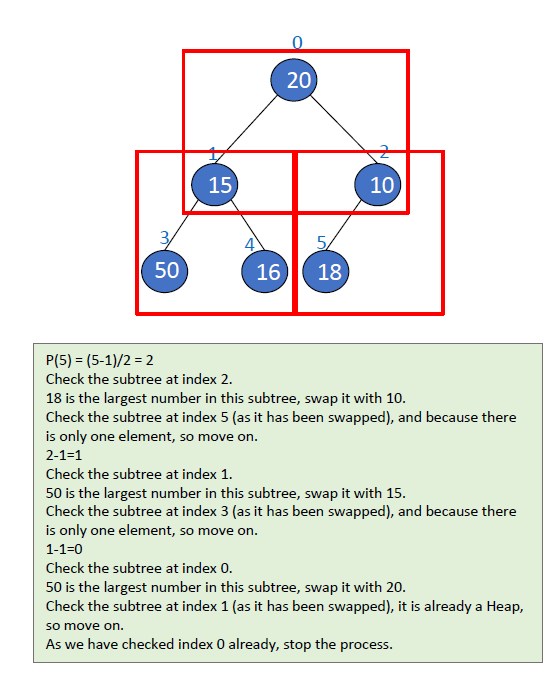
\includegraphics[width=14cm]{unit-5/figures/step_to_build.png}
    % \caption*{Binary Heap}
\end{figure}
\begin{enumerate}
  \item Start from the last parent node and check subtree.
  \item Swap largest node to root of subtree.
  \item Repeat recursively up to the original root.
\end{enumerate}

\textbf{Time Complexity – Build Max-Heap: $O(n)$}

\[
S = \frac{n}{2} \times 0 + \frac{n}{4} \times 1 + \frac{n}{8} \times 2 + \cdots \approx n
\]

\textbf{Heapify}

\begin{itemize}
  \item Start from root.
  \item Compare children and swap with the larger one if needed.
  \item Repeat on the swapped node.
\end{itemize}

\textbf{Time Complexity: $O(\log n)$}
\begin{itemize}
    \item Because half of the tree remains to be a heap, therefore on each level (of the tree), we only need to
swap a single node with one of its children.
    \item In this case, the time complexity is equal to the height of the tree , which is floor $(\log 2(n))$.
\end{itemize}

\subsection{Heapsort Steps}

\begin{enumerate}
  \item Swap root with last node.
  \item Cut and place the last node into sorted array.
  \item Heapify the tree.
  \item Repeat.
\end{enumerate}

\subsection*{Heapsort Time \& Space Complexity}

\begin{itemize}
  \item Heapify: $O(\log n)$ repeated $n$ times.
  \item Build Max-Heap: $O(n)$
  \item \textbf{Overall:} $O(n + n\log n) = O(n\log n)$
  \item Space: $O(1)$
\end{itemize}

\textbf{QuickSort vs MergeSort vs HeapSort}

\begin{center}
\begin{tabular}{|l|c|c|c|c|}
\hline
Name & Average & Worst & Space & Stable \\
\hline
MergeSort & $O(n\log n)$ & $O(n\log n)$ & $O(n)$ & Yes \\
QuickSort & $O(n\log n)$ & $O(n^2)$ & $O(\log n)$ & No \\
HeapSort & $O(n\log n)$ & $O(n\log n)$ & $O(1)$ & No \\
\hline
\end{tabular}
\end{center}


